\documentclass[letter,10pt]{report}
\usepackage{graphics}
\usepackage{graphicx}
\usepackage{amsmath}
\usepackage{amssymb}
\usepackage{color}
\usepackage{verbatim}
\usepackage{hyperref}
%\usepackage{dsfont}


%\usepackage{dsfont}

\setlength{\oddsidemargin}{  0mm}
\setlength{\topmargin}    { -12mm}
\setlength{\textheight}   { 246mm}
\setlength{\textwidth}    { 165mm}
\setlength{\parindent}    {  0   pt}  % not actually required but they
\setlength{\parskip}      {  6   pt}  % make paragraphs look less ugly

\newcommand{\MSbar}{$\overline{MS}$~}
\newcommand{\RIp}{$RI^\prime$~}
\newcommand{\dfk}{\int\frac{d^4k}{(2\pi)^4}}
\newcommand{\ddk}{\mu^\epsilon \int\frac{d^dk}{(2\pi)^d}}
\newcommand{\dfl}{\int\frac{d^4l}{(2\pi)^4}}
\newcommand{\ddl}{\mu^\epsilon \int\frac{d^dl}{(2\pi)^d}}
\newcommand{\mueps}{\mu^\epsilon}
\newcommand{\epstil}{\toe  - \gamma^E + \log 4\pi}
\newcommand{\epshat}{\frac{1}{\hat{\epsilon}}}
\newcommand{\dx}{\int\limits_0^1 dx}
\newcommand{\dy}{\int\limits_0^{1-x} dy}
\newcommand{\s}[1]{\slashed{#1}}
\newcommand{\sk}{\s{k}}
\renewcommand{\sl}{\s{l}}
\renewcommand{\sp}{\s{p}}
\newcommand{\sQ}{\s{Q}}
\newcommand{\spp}{\s{p}^\prime}
\newcommand{\pp}{p^\prime}
\newcommand{\ppp}{p^{\prime 2}}
\newcommand{\hd}{\frac{d}{2}}
\newcommand{\toe}{\frac{2}{\epsilon}}
\newcommand{\half}{\frac{1}{2}}
\newcommand{\ident}{\mathds{1}}
\newcommand{\R}{\mathbb{R}}
\newcommand{\Z}{\mathbb{Z}}
\newcommand{\gm}{\gamma_\mu}
\newcommand{\gn}{\gamma_\nu}
\newcommand{\ga}{\gamma_\alpha}
\newcommand{\gb}{\gamma_\beta}
\newcommand{\Tr}{\mathrm{Tr}}
\newcommand{\beq}{\begin{equation}}
\newcommand{\eeq}{\end{equation}}
\usepackage{slashed}
\pagestyle{headings}

\title{SciDAC-5 Wilson fermion conventions}

\author{Peter A Boyle}

\begin{document}

\maketitle

\tableofcontents

\chapter{Introduction}

This document summarises conventions used in the 
generalised chiral fermion support used in Grid and BFM.

It is quite obviously based on a lot of work by many authors in
the field including Furman, Shamir, the RBC and UKQCD collaborations,
Neuberger, Luscher, Kikukawa, Yamada, 
Borici, Edwards, Heller, Brower, Neff, Joo, Kennedy, Wenger.

I acknowledge access to the Chroma code base with which I have
regressed my code (sometimes with an optional convention transformation).
There are many tests within the tests subdirectory of the BFM 
package which verify that BFM/BAGEL reproduces the corresponding Chroma operator.

\section{Conventions}
First my conventions.

\subsection{Dirac matrices}

The Dirac matrices operate on spin indices of our Fermion fields.
These are $4\times 4$ complex valued matrices forming an anticommuting matrix basis,
that generalises the Quaternions to a larger dimension.

A spinor is a rank 4 spin-vector which is acted upon with these Dirac matrices.

The Dirac matrices statisfy
$$
\gamma_\mu \gamma_\nu + 
\gamma_\nu \gamma_\mu = 2 \delta_{\mu\nu},
$$
and in particular $\gamma_\mu^2 = 1$.

$\gamma_5$ is introduced and anticommutes with all the other Dirac matrices (so they form a totally anticommuting set).

Since a Lorentz vector $p^\mu$ is a commuting scalar while the Dirac matrices anticommute, we have
$$
p_\mu \gamma_\mu 
p_\nu \gamma_\nu  = p_\mu p_\nu \frac{1}{2}\left( \gamma_\mu \gamma_\nu+ \gamma_\nu \gamma_\mu \right) = p_\mu p_\mu = p^2
$$

We will focus initially on the internal indices as these are the building blocks assembled
in Lattice container classes. Every Lattice container class constructor requires a Grid object 
pointer. 

The spin basis is:

$$ \gamma_x= \left(\begin{array}{cccc}    0& 0& 0& i\\  0& 0& i& 0\\  0&-i& 0& 0\\ -i& 0& 0& 0 \end{array}\right)$$

$$ \gamma_y= \left(\begin{array}{cccc}    0& 0& 0&-1\\  0& 0& 1& 0\\  0& 1& 0& 0\\ -1& 0& 0& 0 \end{array}\right)$$

$$ \gamma_z= \left(\begin{array}{cccc}    0& 0& i& 0\\  0& 0& 0&-i\\ -i& 0& 0& 0\\  0& i& 0& 0 \end{array}\right)$$

$$ \gamma_t= \left(\begin{array}{cccc}    0& 0& 1& 0\\  0& 0& 0& 1\\  1& 0& 0& 0\\  0& 1& 0& 0 \end{array}\right)$$

$$ \gamma_5= \left(\begin{array}{cccc}    1& 0& 0& 0\\  0& 1& 0& 0\\  0& 0&-1 &0\\  0& 0& 0&-1 \end{array}\right)$$

Multiplication of a spin vector or matrix can be implemented via subroutines that simply permute data and apply signs.

\subsection{Tensor types}

The Tensor data structures are built up from fundamental 
scalar matrix and vector classes::

\begin{verbatim}
    template<class vobj      > class iScalar { private: vobj _internal ; } 
    template<class vobj,int N> class iVector { private: vobj _internal[N] ; } 
    template<class vobj,int N> class iMatrix { private: vobj _internal[N][N] ; }
\end{verbatim}

These are template classes and can be passed a fundamental scalar or vector type, or
nested to form arbitrarily complicated tensor products of indices. All mathematical expressions
are defined to operate recursively, index by index.

Presently the constants $N_c$ and $N_d$
are globally predefined. However, this is planned for changed in future and policy classes
for different theories (e.g. QCD, QED, SU2 etc...) will contain these constants and enable multiple
theories to coexist more naturally.

Arbitrary tensor products of fundamental scalar, vector
and matrix objects may be formed in principle by the basic Grid code. 

For Lattice field theory, we define types according to the following tensor
product structure ordering. The suffix "D" indicates either double types, and
replacing with "F" gives the corresponding single precision type.

Type definitions are provided in qcd/QCD.h to give the internal index structures
of QCD codes. For example::
\begin{verbatim}
    template<typename vtype> 
    using iSinglet                   = iScalar<iScalar<iScalar<vtype> > >;
    using iSpinMatrix                = iScalar<iMatrix<iScalar<vtype>, Ns> >;
    using iColourMatrix              = iScalar<iScalar<iMatrix<vtype, Nc> > > ;
    using iSpinColourMatrix          = iScalar<iMatrix<iMatrix<vtype, Nc>, Ns> >;
    using iLorentzColourMatrix       = iVector<iScalar<iMatrix<vtype, Nc> >, Nd > ;
    using iDoubleStoredColourMatrix  = iVector<iScalar<iMatrix<vtype, Nc> >, Nds > ;
    using iSpinVector                = iScalar<iVector<iScalar<vtype>, Ns> >;
    using iColourVector              = iScalar<iScalar<iVector<vtype, Nc> > >;
    using iSpinColourVector          = iScalar<iVector<iVector<vtype, Nc>, Ns> >;
    using iHalfSpinVector            = iScalar<iVector<iScalar<vtype>, Nhs> >;
    using iHalfSpinColourVector      = iScalar<iVector<iVector<vtype, Nc>, Nhs> >;
\end{verbatim}

Giving the type table:

\begin{tabular}{cccccc}
\hline
Lattice &  Lorentz &   Spin &   Colour & scalartype & Field \\
\hline
Scalar  &  Scalar &    Scalar & Scalar & RealD     &    RealD \\
Scalar  &  Scalar &    Scalar & Scalar & ComplexD  &    ComplexD \\
Scalar  &  Scalar &    Scalar & Matrix & ComplexD  &    ColourMatrixD \\
Scalar  &  Vector &    Scalar & Matrix & ComplexD  &    LorentzColourMatrixD \\
Scalar  &  Scalar &    Vector & Vector & ComplexD  &    SpinColourVectorD \\
Scalar  &  Scalar &    Vector & Vector & ComplexD  &    HalfSpinColourVectorD \\
Scalar  &  Scalar &    Matrix & Matrix & ComplexD  &    SpinColourMatrixD \\
\hline
\end{tabular}

The types are implemented via a recursive tensor nesting system.

Here, the prefix "i" indicates for internal use, preserving the template nature of the class. 
Final types are declared with vtype selected to be both scalar and vector, appropriate to a
single datum, or stored in a partial SoA transformed lattice object:

\begin{verbatim}
    // LorentzColour
    typedef iLorentzColourMatrix<Complex  > LorentzColourMatrix;
    typedef iLorentzColourMatrix<ComplexF > LorentzColourMatrixF;
    typedef iLorentzColourMatrix<ComplexD > LorentzColourMatrixD;

    typedef iLorentzColourMatrix<vComplex > vLorentzColourMatrix;
    typedef iLorentzColourMatrix<vComplexF> vLorentzColourMatrixF;
    typedef iLorentzColourMatrix<vComplexD> vLorentzColourMatrixD;
\end{verbatim}

Arbitrarily deep tensor nests may be formed. Grid uses a positional and numerical rule to associate indices for contraction
in the Einstein summation sense.

\begin{tabular}{ccc}
\hline
Symbolic name &  Number &  Position\\
\hline
LorentzIndex  &   0 &       left\\
SpinIndex     &   1 &       middle\\
ColourIndex   &   2 &       right\\
\hline
\end{tabular}

The conventions are that the index ordering left to right are: Lorentz, Spin, Colour. A scalar type (either real
or complex, single or double precision) is be provided to the innermost structure.


\subsection{Wilson matrix}

\begin{itemize}
\item $x$ runs over four dimensional cartesian coordinate system, of size $L^3\times T$.
\item $\mu$ is a direction index running from 0 to 3
\item $s$ (where used) is fifth dimensional coordinate of size $L_s$
\item $U_\mu(x)$ is a $3\times 3$ complex color matrix valued gauge field
\item $\psi(x)$ is a $4\times 3$ complex spin-color vector valued Fermion field
\item The Wilson (sparse) matrix operates on this vector space, with elements involving Dirac matrices on spin indices, and color
  matrices on color indices.
\item $M$ is a real valued ``mass''.
\item We use Einstein summation convention where repeated indices are summed over their natural range
\item Color indices use roman letters $i, j, k $ running from 0 to 2
\item Spin indices use Greek letters $\alpha, \beta$ running from 0 to 3
\item Lorentz indices use Greek letters $\mu,\nu$ running from 0 to 3
\end{itemize}

Usual Wilson matrix operates on Fermion spin-colour vector and is
$$D_{W \alpha\beta}^{ij}(x,y) = (M+4)\delta_{\alpha\beta}\delta_{ij}\delta_{x,y} - \frac{1}{2} D_{ {\rm hop}\alpha\beta}^{ij}(x,y),$$ 
where
\begin{equation}
D_{\rm hop \alpha\beta}^{ij}(x,y)\psi^j_\beta(y) = \left[(1-\gamma_\mu)_{\alpha\beta} U^{ij}_\mu(x) \delta_{x+\mu,y} +
                                    (1+\gamma_\mu)_{\alpha\beta} U_\mu^{\dagger ij}(y) \delta_{x-\mu,y} \right]\psi^j_\beta(y)
\end{equation}

\section{Correctness tests}

\subsection{Unit gauge solution by Fourier transform}

Fourier transform

\begin{itemize}
\item coordinate space to momentum space
  $$
  \tilde{F}(p) = \frac{1}{V}\sum_x e^{-i p.x} F(x)
  $$
  \item momentum space to coordinate space
  $$
  F(x)=  \sum_p e^{i p.x} \tilde{F}(p)
  $$
\item CHECK: Resolution of identity with $F(x) = e^{i q.x}$
  $$
  \tilde{F}(p) = \frac{1}{V} \sum_x e^{-i p.x} e^{i q.x} = \delta_{p,q} 
  $$
  $$
  F(x)=  \sum_p e^{i p.x} \delta_{p,q} = e^{i q.x}
  $$
\end{itemize}

\href{https://github.com/paboyle/Grid/blob/develop/tests/core/Test\_fft\_matt.cc}{https://github.com/paboyle/Grid/blob/develop/tests/core/Test\_fft\_matt.cc}

The Wilson operator in the free field (U=1) is translation invariant: $$D_W(x,y) = D_W(x-y)$$

The (two coordinate) Fourier transform of a translation invariant matrix takes simple form and leads to a momentum conserving delta:
\begin{eqnarray}
 \frac{1}{V^2} \sum_{xy}  e^{-iqx} e^{ipy} D_{xy}
 &=&  
\frac{1}{V^2} \sum_{xy}  e^{-iqx} e^{ipy} D(x-y)\\
 &=& \frac{1}{V^2} \sum_{xu} e^{-iqx} e^{ip(x-u)} D(u)\\
= \frac{1}{V^2} \sum_{xu} e^{i(p-q)x} e^{-ip(u)} D(u)\\
= \delta_{p,q} \tilde{D}(p)
\end{eqnarray}

Application of $D_W$ is therefore a convolution,
$$
D_W(x,y) \psi(y) = \sum_y D_W(x-y) \psi(y)
$$

$$
\tilde{D}_W(p) = \frac{1}{V} \sum_x D_W(x) e^{-ipx}
$$

Convolution theorem for this norm of FT is:
\begin{eqnarray}
  \sum_y F(x-y) G(y)
&=&
 \sum_{p,q}  \sum_y\tilde{F}(p) \tilde{G}(q)e^{i p.(x-y)}e^{i q.(y)}\\
&=&
 \sum_{p,q}  \tilde{F}(p) \tilde{G}(q)e^{i p.x} \sum_y e^{i (q-p).(y)}\\
&=&
 \sum_{p,q}  \tilde{F}(p) \tilde{G}(q)e^{i p.x} V \delta_{p,q}\\
&=&
 \sum_{p}  V \tilde{F}(p) \tilde{G}(p) e^{i p.x} \\
&=&
 \sum_{p}  \tilde{C}(p) e^{i p.x} 
\end{eqnarray}

Thus we can identify the Fourier transform of the convolution $C = F \ast G$ as
$$\tilde{C}(p)=V \tilde{F}(p) \tilde{G}(p)$$

We can Fourier transform the Wilson matrix $D_W$ in the left and right variables with $U_\mu=1$.
\begin{eqnarray}
  D_W(p)
  &=&  
\frac{1}{V^2}  \sum\limits_{x,y} e^{-i q.x}e^{i p.y} D_W(x-y)\\
  &=& 
\frac{1}{V^2}
\sum\limits_{x}
e^{i(p-q).x} \left[ (M+4) - \sum_\mu
e^{ip_\mu} \frac{1}{2}(1-\gamma_\mu)
+e^{-ip_\mu} \frac{1}{2}(1+\gamma_\mu) \right]\\
  &=& 
\frac{1}{V}\delta_{q,p} \left( M + \sum_\mu (1-\cos p_\mu) + i \gamma_\mu \sin p_\mu \right)\\
  &=& 
  \label{Eq:DWp}
\frac{1}{V}
\delta_{q,p} \left( M + \sum_\mu 2 \sin^2 \frac{p_\mu}{2} + i \gamma_\mu \sin p_\mu \right)
\end{eqnarray}

Thus, coordinate space multiplication by $D_W$ (i.e. a convolution with $D_W$) reduces to multiplication in Fourier space by
$$
\left( M + \sum_\mu 2 \sin^2 \frac{p_\mu}{2} + i \gamma_\mu \sin p_\mu \right)
$$
This is also relatively easy to invert, and the inverse is
$$
\frac{M+\sum_\mu  2 \sin^2 \frac{p_\mu}{2} -i \gamma_\mu \sin p_\mu }{ \sum_\mu \sin^2 p_\mu + (2 \sum_\mu \sin^2 \frac{p_\mu}{2} + m)^2 }
$$

\subsubsection{Check 1: Wilson matrix check}

Thus a convenient first test for a new code for $D_w(x,y)$ is to
\begin{itemize}
  \item Pick a random vector $b$
  \item apply the coordinate space operator $D_w b$
  \item Fourier transform the result to obtain $\tilde{\psi}(p)$
  \item Fourier transform to obtain $\tilde{b}(p)$
  \item Multiply by $D_W(p)$ to obtain $D_W(p) \tilde{b}(p)$ Eq~\ref{Eq:DWp}
  \item Compare $ D_W(p) b(p)$ to $\tilde{\psi}(p)$
\end{itemize}

See Lines 82-138 of:
\href{https://github.com/paboyle/Grid/blob/develop/tests/core/Test\_fft\_matt.cc}{https://github.com/paboyle/Grid/blob/develop/tests/core/Test\_fft\_matt.cc}

\begin{verbatim}
    RealD mass=0.1;
    WilsonFermionD Dw(Umu,GRID,RBGRID,mass);
    
    Dw.M(src,ref);
    std::cout << "Norm src "<<norm2(src)<<std::endl;
    std::cout << "Norm Dw x src "<<norm2(ref)<<std::endl;
    {
      FFT theFFT(&GRID);

      ////////////////
      // operator in Fourier space
      ////////////////
      tmp =ref;
      theFFT.FFT_all_dim(result,tmp,FFT::forward);
      std::cout<<"FFT[ Dw x src ]  "<< norm2(result)<<std::endl;    

      tmp = src;
      theFFT.FFT_all_dim(src_p,tmp,FFT::forward);
      std::cout<<"FFT[ src      ]  "<< norm2(src_p)<<std::endl;
      
      /////////////////////////////////////////////////////////////////
      // work out the predicted FT from Fourier
      /////////////////////////////////////////////////////////////////
      auto FGrid = &GRID;
      LatticeFermionD    Kinetic(FGrid); Kinetic = Zero();
      LatticeComplexD    kmu(FGrid); 
      LatticeInteger     scoor(FGrid); 
      LatticeComplexD    sk (FGrid); sk = Zero();
      LatticeComplexD    sk2(FGrid); sk2= Zero();
      LatticeComplexD    W(FGrid); W= Zero();
      LatticeComplexD    one(FGrid); one =ComplexD(1.0,0.0);
      ComplexD ci(0.0,1.0);
    
      for(int mu=0;mu<Nd;mu++) {
        LatticeCoordinate(kmu,mu);
        RealD TwoPiL =  M_PI * 2.0/ latt_size[mu];
        kmu = TwoPiL * kmu;
        sk2 = sk2 + 2.0*sin(kmu*0.5)*sin(kmu*0.5);
        sk  = sk  +     sin(kmu)    *sin(kmu); 
        Kinetic = Kinetic + sin(kmu)*ci*(Gamma(Gmu[mu])*src_p);
      }
    
      W = mass + sk2; 
      Kinetic = Kinetic + W * src_p;
    
      std::cout<<"Momentum space src         "<< norm2(src_p)<<std::endl;
      std::cout<<"Momentum space Dw x src    "<< norm2(Kinetic)<<std::endl;
      std::cout<<"FT[Coordinate space Dw]    "<< norm2(result)<<std::endl;
    
      result = result - Kinetic;
      std::cout<<"diff "<< norm2(result)<<std::endl; // Should be zero up to rounding
    }
\end{verbatim}

This test passes:
\begin{verbatim}
./Test_fft_matt --grid 8.8.8.16
---
Grid : Message : 0.163137 s : Grid is setup to use 1 threads
Norm src 196235
Norm Dw x src 4.07469e+06
FFT[ Dw x src ]  3.33799e+10
FFT[ src      ]  1.60756e+09
Momentum space src         1.60756e+09
Momentum space Dw x src    3.33799e+10
FT[Coordinate space Dw]    3.33799e+10
diff 3.61034e-21
\end{verbatim}

\subsubsection{Check 2: Wilson matrix check}

Grid also implements the inverse of the free Wilson operator via convolution.
using equation~\ref{Eq:DWip}.
A related check is that the Fourier based inverse  (Greens function) indeed
inverts the coordinate space operator we have coded up as $D_w$.

\begin{verbatim}
    std::cout << " =======================================" <<std::endl;
    std::cout << " Checking FourierFreePropagator x Dw = 1" <<std::endl;
    std::cout << " =======================================" <<std::endl;
    std::cout << "Dw src = " <<norm2(src)<<std::endl;
    std::cout << "Dw tmp = " <<norm2(tmp)<<std::endl;
    Dw.M(src,tmp);
    Dw.FreePropagator(tmp,ref,mass);

    std::cout << "Dw ref = " <<norm2(ref)<<std::endl;
    
    ref = ref - src;
    
    std::cout << "Dw ref-src = " <<norm2(ref)<<std::endl;
\end{verbatim}

This test passes:
\begin{verbatim}
 =======================================
 Checking FourierFreePropagator x Dw = 1
 =======================================
Dw src = 196235
Dw tmp = 196235
Dw ref = 196235
Dw ref-src = 3.32075e-26
\end{verbatim}


\subsection{Specific volume/mass results}

\subsubsection{Check 3: full solver check}

We can check solvers on the free field using 
Fourier convolution and equation~\ref{Eq:DWip}.

$$
D_W \psi = b \iff \tilde\psi(p) = D_W^{-1}(p) \tilde{b}(p)
$$

This can of course be FT'd back to coordinate space and the check applied directly on the result
of a Krylov or multigrid solver. See the above file linked for examples.

\begin{verbatim}
    LatticeFermionD    src(&GRID); gaussian(pRNG,src);
    LatticeFermionD    tmp(&GRID);
    LatticeFermionD    ref(&GRID);
    LatticeFermionD    diff(&GRID);

    src=Zero();
    Coordinate point(4,0); // 0,0,0,0
    SpinColourVectorD ferm;
    ferm=Zero();
    ferm()(0)(0) = ComplexD(1.0);
    pokeSite(ferm,src,point);

    RealD mass=0.1;
    WilsonFermionD Dw(Umu,GRID,RBGRID,mass);

    // Momentum space prop
    std::cout << " Solving by FFT and Feynman rules" <<std::endl;
    Dw.FreePropagator(src,ref,mass) ;

    LatticeFermionD    result(&GRID); 
    
    ////////////////////////////////////////////////////////////////////////
    // Conjugate gradient on normal equations system
    ////////////////////////////////////////////////////////////////////////
    std::cout << " Solving by Conjugate Gradient (CGNE)" <<std::endl;
    Dw.Mdag(src,tmp);
    src=tmp;
    MdagMLinearOperator<WilsonFermionD,LatticeFermionD> HermOp(Dw);
    ConjugateGradient<LatticeFermionD> CG(1.0e-10,10000);
    CG(HermOp,src,result);
    
    ////////////////////////////////////////////////////////////////////////
    std::cout << " Taking difference" <<std::endl;
    std::cout << "Dw result "<<norm2(result)<<std::endl;
    std::cout << "Dw ref     "<<norm2(ref)<<std::endl;
    
    diff = ref - result;
    std::cout << "result - ref     "<<norm2(diff)<<std::endl;

    DumpSliceNorm("Slice Norm Solution ",result,Nd-1);
\end{verbatim}

We take an $8^3 \times 16$ the $N_c=3$ Wilson action with input mass 0.1 and either unit gauge links
or gauge links that are a random gauge transform of unity.

The source is a kronecker delta in space, spin and colour: $b_\beta^j(y)=\delta_{y,0}\delta_{j,0}\delta_{\beta,0}$,
so contains a single real number 1 in the first element and zero everywhere else.

We compute by FFT as described above that the solution should have timeslice by timeslice norm, and obtain:

\begin{verbatim}
****************************************
Wilson Mom space 4d propagator 
****************************************
 Solving by FFT and Feynman rules
 Solving by Conjugate Gradient (CGNE)
Grid : Message : 13.988509 s : ConjugateGradient Converged on iteration 110	Computed residual 6.4878e-11	True residual 6.4879e-11	Target 1e-10
 Taking difference
Dw result 0.0918289
Dw ref     0.0918289
result - ref     1.77143e-21
Slice Norm Solution  0 S {S {S {(0.0708605,0)}}}
Slice Norm Solution  1 S {S {S {(0.00509478,0)}}}
Slice Norm Solution  2 S {S {S {(0.00151241,0)}}}
Slice Norm Solution  3 S {S {S {(0.000945715,0)}}}
Slice Norm Solution  4 S {S {S {(0.000767837,0)}}}
Slice Norm Solution  5 S {S {S {(0.000674655,0)}}}
Slice Norm Solution  6 S {S {S {(0.000617168,0)}}}
Slice Norm Solution  7 S {S {S {(0.000584637,0)}}}
Slice Norm Solution  8 S {S {S {(0.000574033,0)}}}
Slice Norm Solution  9 S {S {S {(0.000584637,0)}}}
Slice Norm Solution  10 S {S {S {(0.000617168,0)}}}
Slice Norm Solution  11 S {S {S {(0.000674655,0)}}}
Slice Norm Solution  12 S {S {S {(0.000767837,0)}}}
Slice Norm Solution  13 S {S {S {(0.000945715,0)}}}
Slice Norm Solution  14 S {S {S {(0.00151241,0)}}}
Slice Norm Solution  15 S {S {S {(0.00509478,0)}}}
\end{verbatim}


This should be true on either a unit gauge configuration or a random gauge transform of the unit gauge configuration.
Next section will discuss enhanced tests with non-trivial gauge links.

\subsection{Lie algebra, Lie group and random gauge fields}

In order to perform random gauge transforms we must create random elements of the SU(3) special (${\rm det}g=1$) unitary ($g^\dagger g = 1$) group.

This is simplest to perform in the Lie algebra su(3) of the group SU(3).

We take eight real valued Gaussian random fields $\lambda^a(x)$ and write $\Lambda(x) = \lambda^a(x) T^a$
and
$$
g(x) = e^{i\lambda^a(x) T^a} = \sum_{n=0}^{12} \frac{1}{n!} \Lambda(X)^n 
$$
Where in practice a 12th order Taylor expansion is sufficent since $\Lambda$ is bounded and $12 !$ is large.

Here, the generators $T^a$ are related to the Gell Mann matrices and are:
$$
T^0 =
\frac{1}{2} \left(
\begin{array}{ccc}
0  & i & 0 \\
-i  & 0 & 0\\
0  & 0 & 0
  \end{array}\right)
$$

$$
T^1 =
\frac{1}{2} \left(
\begin{array}{ccc}
0  & 1 & 0 \\
1  & 0 & 0\\
0  & 0 & 0
  \end{array}\right)
$$
$$
T^2 =
\frac{1}{2} \left(
\begin{array}{ccc}
0  & 0 & i \\
0  & 0 & 0\\
-i  & 0 & 0
  \end{array}\right)
$$
$$
T^3 =
\frac{1}{2} \left(
\begin{array}{ccc}
0  & 0 & 1 \\
0  & 0 & 0\\
1  & 0 & 0
  \end{array}\right)
$$
$$
T^4 =
\frac{1}{2} \left(
\begin{array}{ccc}
0  & 0 & 0 \\
0  & 0 & i\\
0  & -i & 0
  \end{array}\right)
$$

$$
T^5 =
\frac{1}{2} \left(
\begin{array}{ccc}
0  & 0 & 0 \\
0  & 0 & 1\\
0  & 1 & 0
  \end{array}\right)
$$
$$
T^6 =
\frac{1}{2} \left(
\begin{array}{ccc}
1  & 0 & 0 \\
0  & -1 & 0\\
0  & 0 & 0
  \end{array}\right)
$$
$$
T^7 =
\frac{1}{2} \left(
\begin{array}{ccc}
\frac{1}{\sqrt{3}}  & 0 & 0 \\
0  & \frac{1}{\sqrt{3}} & 0\\
0  & 0 & -\frac{2}{\sqrt{3}}
  \end{array}\right)
$$

\subsection{Free Wilson eigenvalues}

As shown above, due to translational invariance, the free Wilson matrix is diagonal in Fourier space,
\begin{eqnarray}
 \frac{1}{V^2} \sum_{xy}  e^{-iqx} e^{ipy} D_{xy}
= \delta_{p,q} \tilde{D}(p),
\end{eqnarray}
where
$$
\tilde{D}(p) = \left( M + \sum_\mu 2 \sin^2 \frac{p_\mu}{2} + i \gamma_\mu \sin p_\mu \right)
$$

We can easily compute the eigenvalues of $D(p)$ and hence those of free Wilson fermions.

The term proportional to the identity, $ M + \sum_\mu 2 \sin^2 \frac{p_\mu}{2}$ dictates the real part of the
eigenvalues, while the eigenvectors are dictated by the eigenvalue equation of the non-diagonal term,

$$
i \gamma_\mu \sin p_\mu \psi = \alpha \psi
$$
Recalling $ a_\nu \gamma_\nu a_\mu \gamma_mu = a^2$ arises from the anti-commutavity and squaring to one property
of the Euclidean Dirac matrices, we see that multiplying by $i \gamma_\nu \sin p_\nu $ we have

$$
i^2 \gamma_\nu \sin p_\nu \gamma_\mu \sin p_\mu \psi = i^2 \left(\sum_\mu \sin^2 p_\mu\right) =   i \gamma_\nu \sin p_\nu \alpha \psi = \alpha^2 \psi,
$$
and so
$$
\alpha^2 = - \left(\sum_\mu \sin^2 p_\mu\right)
$$
and the eigenvalue $\lambda_i$ of the Dirac matrix portion of the Wilson term is imaginary with $\lambda_i = \pm i \sqrt{\sum_\mu \sin^2 p_\mu }$.

The possible eigenvalues for each Fourier momentum mode $p$ are thus
$$
\lambda_p = \lambda_r + \lambda_i = \left( M + \sum_\mu 2 \sin^2 \frac{p_\mu}{2} \pm  i \sqrt{\sum_\mu \sin^2 p_\mu } \right)
$$


\subsection{Gauge invariance}

The (energy) action is invariant under a local redefintion of the fields $U_\mu(x)$ and $\psi(x)$.

In the case of U(1) gauge theory this is equivalent to the phase of a quantum mechanical wave function being unobservable,
but when the electromagnetic vector potential can be redefined a local phase can be absorbed.

We introduce a free (randomly chosen) gauge rotation matrix $$g(x) \in SU(3)$$ so that $$ g^\dagger(x) g(x) = 1 \forall x$$.
The action is gauge invariant if we \emph{transform} simultaneously transform $U_\mu(x)$ and $\psi(x)$ as follows:

$$U_\mu(x) \to U_\mu^\prime(x) = g(x) U_\mu(x) g^\dagger(x+\mu)$$

$$\psi(x) \to \psi^\prime(x) = g(x) \psi(x)$$

Fermion fields live on nodes of the grid and transform in the fundemental representation of SU(3).
Gauge fields live on edges of the grid and transform in the adjoint representation of SU(3).
The gauge links are gauge covariant parallel transporters along an edge of the cartesian grid.

\subsubsection{sketch}
Consequently,
\begin{itemize}
\item Any path made out of naturally connecting products of $\psi^\dagger$, $\psi$ and gauge links $U$ is invariant:
$$\psi^\dagger U_1 U_2 \ldots U_n \psi \to \psi^\dagger g^\dagger g U_1 g^\dagger g U_2  g^\dagger g \ldots   g^\dagger g U_n g^\dagger g \psi =
 \psi^\dagger U_1 U_2 \ldots U_n \psi$$
\item Any trace of a closed loop of gauge links is invariant:
  $$
  {\rm Tr}\left[ U_1 U_2 \ldots U_n \right] \to   {\rm Tr}\left[g^\dagger U_1 g^\dagger g U_2 g^\dagger g \ldots g^\dagger U_n g \right]
  $$
were all factors of $g^\dagger g = 1$ and using the cyclic property of the trace.
\end{itemize}

In particular, the local (and hence global) site norm of a Fermion field $\psi$ is invariant under a gauge transform,
since $\psi^\dagger(x) \psi(x) \to \psi^\dagger(x) g(x)^\dagger g(x) \psi = \psi^\dagger(x) \psi(x)$

Thus, the solution from a point source right hand side has a norm that is gauge invariant, and can be computed by Fourier
transform on a unit gauge, but the time-sliced norm does not change if instead computed on a \emph{random} gauge transform
of the unit gauge.

We compute by FFT as described above that the solution should have timeslice by timeslice norm as follows on $8^3\times 16$ with a
mass of $m=0.1$.

\begin{verbatim}
0 0.0708605
1 0.00509478
2 0.00151241
3 0.000945715
4 0.000767837
5 0.000674655
6 0.000617168
7 0.000584637
8 0.000574033
9 0.000584637
10 0.000617168
11 0.000674655
12 0.000767837
13 0.000945715
14 0.00151241
15 0.00509478
\end{verbatim}

This provides an excellent and robust test of the code with non-trival coefficient data.


\section{Known properties of the non-Free $D_W$ eigenvectors/eigenvalues}

The spectrum of the gauged Wilson operator is only tractable numerically.

However there are known properties to the spectrum which we derive/explain here.

\subsection{$\gamma_5$ Hermiticity}

The $D_w$ operator has $\gamma_5$ Hermiticity, because $\gamma_5$ anticommutes with the other Dirac matrices and due to the
structure of the Wilson operator.

The adjoint is
\begin{eqnarray}
  D_W(x,y) &=& (M+4)\delta_{x,y} - \frac{1}{2}\left( \delta_{y,x+\mu} (1-\gamma_mu) U(x,y)  + \frac{1}{2} \delta_{y,x-\mu} (1+\gamma_mu) U^\dagger(y,x) \right)\\
  D_W^\dagger(y,x)
  &=& (M+4)\delta_{y,x} - \frac{1}{2}\left( \delta_{y,x+\mu} (1-\gamma_mu) U^\dagger(y,x)  + \frac{1}{2} \delta_{y,x-\mu} (1+\gamma_mu) U^\dagger(y,x) \right)\\
  &=& (M+4)\delta_{x,y} - \frac{1}{2}\left( \delta_{x,y-\mu} (1-\gamma_mu) U(x,y)  + \frac{1}{2} \delta_{x,y+\mu} (1+\gamma_mu) U(x,y) \right)\\
  &=& (M+4)\delta_{x,y} - \frac{1}{2}\left( \frac{1}{2} \delta_{x,y+\mu} (1+\gamma_mu) U(x,y) + \delta_{x,y-\mu} (1-\gamma_mu) U(x,y)  \right)\\
  &=&  \gamma_5 D_W(x,y) \gamma_5
\end{eqnarray}

{\bf Thus, because $\gamma_5$ anticommutes with the xyzt Dirac matrces, 
we can implement the adjoint operator by merely flipping the signs of the Dirac matrices in $D_W$.}

With this we see that the operator
$
H_W = \gamma_5 D_W 
$
is Hermitian 
($
H_W^\dagger =  D_W^\dagger \gamma_5 =  \gamma_5 D_W\gamma_5\gamma_5 =  \gamma_5 D_W = H_W
$).


We denote right eigenvectors of $D_W$ as $\phi_i$ and $H_W$ as $\chi_i$,
satisfying,
$$
D_W \phi_i = \lambda_i \phi_i,
$$
and
$$
H_W \chi_i = \mu_i \chi_i,
$$

\subsection{Shifted spectrum}

If the massless Wilson eigenvectors are $\phi_i$, given by
$$
D_W(m=0) \phi_i = \lambda^0 \phi_i
$$
Then the massive Wilson operator $D_W(m)$ obviously has the same eigenvectors $\phi_i$ and eigenvalues $\lambda^m_i = \lambda_0^i+m$.

A consequence of this is that any real eigenvalue becomes a zero eigenvalue for some mass parameter $m=-\lambda_i^0$.

If $D_W(m) \phi = 0$ then $\gamma_5 D_W(m) \phi = 0$ so zero modes of $D_W$ and $H_W$ coincide. By continuity arguments their near null-spectrum
must be similar.

\subsection{Pairing of complex eigenvalues}

Consider an eigenvector
\begin{eqnarray}
  D \phi &=& \lambda_i \phi \\
\Rightarrow  \gamma_5 D \gamma_5^2 \phi= \lambda_i \gamma_5 \phi\\
\Rightarrow   D^\dagger \gamma_5 \phi= \lambda_i \gamma_5 \phi\\
\Rightarrow   \phi^\dagger \gamma_5 D = \lambda_i^\ast  \phi^\dagger \gamma_5\\
\Rightarrow   {\rm det} \left( D - \lambda_i^\ast I \right) = 0
\end{eqnarray}

Since right and left eigenvalues are the same (eigenvectors differ in a non-hermitian operator), we see
that if $\lambda_i$ is complex (has non-zero imaginary component) then $\lambda_i^\ast$ is ALSO an eigenvalue.

\subsection{$\gamma_5$ orthogonality of eigenvalues}

Consider two right eigenvectors $\phi_i$ and $\phi_j$ with eigenvalues $\lambda_i$ and $\lambda_j$
\begin{eqnarray}
  \phi_i^\dagger \gamma_5 D \phi_j &=& \lambda_i^\ast \phi_i^\dagger \gamma_5 \phi_j\\
  &=& \lambda_j \phi_i^\dagger \gamma_5 \phi_j
\end{eqnarray}
So,
$$
(\lambda_i^\ast - \lambda_j)   \phi_i^\dagger \gamma_5 \phi_j = 0
$$
and either
$$
\lambda_i^\ast = \lambda_j 
$$
OR
$$
\phi_i^\dagger \gamma_5  \phi_j = 0
$$

When $i=j$ we see that either the eigenvalue is real and $\phi_i^\dagger \gamma_5 \phi_j \ne 0$ is allowed,
or the eigenvalue has non-zero imaginary part and $\phi_i^\dagger \gamma_5 \phi_j = 0$.

In other words:
\begin{itemize}
\item complex eigenvalues have zero chirality and come in conjugate pairs
\item real eigenvalues in general have non-zero chirality $\chi = \phi_i^\dagger \gamma_5 \phi_i$
\item Eigenvectors with unrelated eigenvalues have vanishing chiral inner product $\phi_i^\dagger \gamma_5 \phi_j = 0$
\end{itemize}


\subsection{$\gamma_5$ symmetry, singular value decomposition and the normal equations}

Suppose $D_W$ has right eigenvectors $R_i$ such that,
$$
D_W R_i = \lambda_i R_i,
$$
or in matrix notation with diagonal matrix $\Lambda$ of eigenvalues:
$$
D_W R = R \Lambda.
$$
Assuming $R$ is invertible (i.e. assuming $D_W$ is not a defective matrix) we have,
$$
D_W = R \Lambda R^{-1}
$$
The columns of R are not necessarily mutually orthogonal. The inverse $R^{-1}$ resolves
linear combinations of non-orthogonal eigenvectors, such as $a R_1 + b R_2$ into the fundamental
$a$ and $b$ components.

% R_ij delta_jk lambda_k multiplis the k-th column of R by lambda_k as needed

The left eigenvectors are such that
$$
L_i^\dagger D_W = \lambda_i L_i^\dagger, 
$$
and,
$$
L^\dagger D_W = \Lambda L^\dagger.
$$

As noted above, the left eigenvectors can be related to right eigenvectors with the complex conjugate eigenvalue via $\gamma_5$ hermititicy:
\begin{eqnarray}
  L \Lambda^\dagger &=& D_W^\dagger L = \gamma_5 D_W \gamma_5 L \\
  D_W \gamma_5 L &=& \gamma_5 L \Lambda^\dagger,
\end{eqnarray}
implying that $\gamma_5 L = R$.

The action of $\gamma_5$ transforms a left eigenvector with eigenvalue $\lambda$ into a right eigenvector with eigenvalue $\lambda^\ast$.
If $\lambda_i$ is complex then the left eigenvector for $\lambda_i$ and right eigenvector for $\lambda_i^\ast$ are related by $\gamma_5$.
If $\lambda_i$ is real then the corresponding left and right eigenvectors are related by $\gamma_5$.

If we build a multigrid subspace that preserves the action of $\gamma_5$ then... WHAT IS BETTER!
(There's been debate between Luscher and US MG folks about $\gamma_5$ compatible coarsening being better -- read up).
(Evan alluded to instanton preservation in his talk)

The {\bf singular value decomposition} of $D_W$ is,
$$
D_W = U \Sigma V^\dagger,
$$
where there is a remnant phase abiguity between rows of $U$ and $V$.

The singular value decomposition of the Hermitian Wilson operator  $\gamma_5 D_W$ is
almost identical to its eigendecomposition, and is simply related,
$$
H_W = V \tilde\Sigma V^\dagger = (\gamma_5 U) \Sigma V^\dagger,
$$
and since $H_W$ is Hermitian we see that $\gamma_5 U = {\rm sgn}(\tilde\Sigma) V$,
where the sign of the (indefinite) eigenvalues of $H_W$ relates the positive
valued $\Sigma$ from the SVD of $D_W$ to the signed eigenvalues of $H_W$.

For the squared Dirac operator, these signs are removed and manifest positivity results
$$
D_W^\dagger D_W = H_W^2 = V (\Sigma)^2 V^\dagger,
$$
$$
D_W D_W^\dagger = \gamma_5 H_W^2 \gamma_5= U (\Sigma)^2 U^\dagger.
$$

The singular values and absolute values of the eigenvalues of $H_W$ are necessarily the same as the singular values of $D_W$ (but differ from the eigenvalues of $D_W$). They are trivially
related to the singular values of the squared operator.


\subsection{Near null vectors}

With (hypothetical) exact null vectors $D_W \psi = 0 = \gamma_5 D_W \psi = D_W^\dagger D_W \psi$, we expect:
\begin{itemize}
  \item $D_W$ has an exact zero right eigenmode, $\psi \in R$ (where ``in'' means is a column of)
  \item $\gamma_5 \psi$ is the corresponding left zero eigenmode
  \item The SVD of $D_W$ \emph{also} has a corresponding exactly zero singular value
        with $\psi \in V$.
  \item $|\gamma_5 \psi \rangle (\sigma=0) \langle \psi |$ is the corresponding null element of the SVD expansion with zero singular value (notation abuse).
\end{itemize}

This equivalence arises only algebraically for exact zero modes.
The question arises whether near null singular values and singular vectors can be used
to set up a non-Hermitian multigrid.

This may ``obviously'' be the case for an SVD based multigrid.

If we generate a space in the ``V'' space and make a $\gamma_5$ compatible coarsening (doubling the space to include
both $V$ and $\gamma_5 V$, then the ``U'')


\subsection{Singular value decomposition deflation and multigrid}

A second approach to deflation, and potentially a novel
approach to multigrid in the non-hermitian  case, is
based on the singular value decomposition:
$$
D = U \Sigma V^\dagger,
$$
where $\Sigma = {\rm diag} (\sigma_i)$ is diagonal real, positive and $U$ and $V$ are unitary. The diagonal elements are the positive square roots
of the eigenvalues of the squared operator.
$$
D^\dagger D = V {\rm diag} (|\sigma_i|^2) V^\dagger
$$
$$
D D^\dagger = U {\rm diag} (|\sigma_i|^2) U^\dagger
$$
These may be solved by using Lanczos to find the eigenpairs
of the hermitian positive
definite problem for either $D^\dagger D$ or $D D^\dagger$.
Once $V$ and $\Sigma$ have been found, $U$ may be constructed
via the application of $D$, 
$$
D V = U \Sigma,
$$
though in practice with approximate eigenvectors a Lanczos restart my be preferable to retain convergence
precision.
Within a truncated subspace we can solve for a deflated guess via
$$
U \Sigma V^\dagger x = r_0
$$
with 
$$
x = \sum_i |v_i\rangle \frac{\langle u_i| r_0\rangle}{\sigma_i}.
$$
This suggests a potential new class of lattice multigrid methods based on the
singular value decomposition, rather than right eigenvectors.

The restriction operator can be based on a block projection of the
$V$ vectors and prolongation on $U$. The matrix elements can be computed
$$
C^{ii^\prime}_{bb^\prime} = U^\dagger_b D V_{b^\prime}
$$

The filtering task of finding $V$ (and $U$) is over the real domain of singular
values rather than a complex spectrum, and may allow better setup methods
than inverse iteration.

{\bf does this have overlap with the staggered MG coarse grid approaches? Saw reference to SVD deflation in
  Evan's talk at CERN
  (I previously wrote this 
  \href{https://www.overleaf.com/read/vqywyddshbnr#b87e9e}{here}
  )
}

\subsection{Mathworks example matrix}

We know that the real spectrum of $H_W$ and complex spectrum of $D_W$ differ massively, as do their eigenvectors.
The exact zeros must coincide, however.

c.f. Saul Cohen's animation of $\Gamma_5^{\epsilon} D_{dwf}$ for $epsilon \in [0,1]$

Useful document by CTO of Mathworks (Matlab) Cleve Moler:

\href{https://www.mathworks.com/content/dam/mathworks/mathworks-dot-com/moler/eigs.pdf}{https://www.mathworks.com/content/dam/mathworks/mathworks-dot-com/moler/eigs.pdf}

$$
A = \left( \begin{array}{ccc}
 -149 & -50 & -154 \\
 537  & 180 & 546 \\
 -27  & -9  & -25
\end{array}
\right) =  X \Lambda X^{-1}
$$
Eigenvalues
$$
\Lambda ={\rm diag}(1,2,3)
$$
Singular values
$$
\Sigma = {\rm diag}(817.7597,2.4750,0.0030)
$$
Eigenvectors
$$
X = \left( \begin{array}{ccc}
 1  & -4 & 7 \\
-3  & 9 & -49 \\
 0  & 1  & 9
\end{array}
\right)
$$
$$
X^{-1} = \left( \begin{array}{ccc}
 130  & 43 & 133 \\
 27  & 9 & 28  \\
 -3  &-1  & -3
\end{array}
\right)
$$

Peturbation analysis on matrix; introduces \emph{eigenvalue condition number} for left (y) and right (x) eigenvectors
$$
1\le \kappa(\lambda,A) = \frac{||y_\lambda|| ||x_\lambda||}{ \langle y_\lambda|x_\lambda \rangle} = \frac{1}{\cos \theta_{xy}}
$$
This factor is always 1 for Hermitian matrices, and amplifies the numerical uncertainty on the eigenvalue for increasingle non-Hermitian


\subsection{$PV^\dagger M$ deflation}


Use variable preconditioned GCR. Equivalent to Flexible GMRES up to rounding.
Minimises the residual norm, difference is in orthonormal basis vs. $A^\dag A$ orthogonal basis of search directions.
(Saad's paper on GMRES says ``theoretically equivalent'').

{\bf Singular vector setup }

\begin{itemize}
\item $P^\dagger M = U \Sigma V^\dagger$
\item First attempted Chebyshev set up in $M^\dagger P P^\dagger M = V \Sigma^\dagger \Sigma V^\dagger$
\item Produces a polynomial of singular values and vectors  
\item Measure ``nulliness'' of singular vector (squared operator): $\langle v | M^\dagger P^{\dagger} M | v \rangle \in \mathbb{C} $  has magnitude around $0.3$
\item Measure ``nulliness'' of wrt. eigenvector subspace: $\langle v | P^{dag} M | v \rangle \in \mathbb{C} $ has magnitude around $0.2$
  \begin{itemize}
  \item $U$ / $V$ space misalignment might have made this worse!
  \end{itemize}
\item Chebyshev parameters lowpass of order 0.1, filter orders 400.. 1800
\item Coarse solver, smoother (low pass GCR 16 iters, shift 1.0
\item Solver converged, but deflation effect negligible - around 350 outer iterations
\item Will revisit singular vector space setup
\end{itemize}
  
{\bf Eigenvector setup }
\begin{itemize}
\item Produce vectors by inverse iteration 2/3/4 steps with sloppy solves
\item $P^\dagger M = R \Lambda R^{-1}$
\item Measure ``nulliness'' of wrt. eigenvector subspace: $\langle v | P^{dag} M | v \rangle \in \mathbb{C} $ has magnitude around $0.008$
\item Solver converges with real deflation effect around 50 outer iterations
\item Playing with number of vectors (8 - 24), block size solver parameters ($4^4$, $2^4$)
\end{itemize}


\section{Optimised implementation}

Following sections are implementation notes for optimisation and benchmarking of a matrix free implementation to usual
standards in the field.

\subsubsection{Spin projection optimisation}

\href{https://github.com/paboyle/Grid/blob/develop/Grid/qcd/spin/TwoSpinor.h}{https://github.com/paboyle/Grid/blob/develop/Grid/qcd/spin/TwoSpinor.h}

The matrix $P^\pm_\mu = \frac{1}{2} (1\pm\gamma_\mu)_{\alpha\beta}$ is a projector,
$$(P^\pm_\mu)^2 =  \frac{1}{4} (1\pm\gamma_\mu)(1\pm\gamma_\mu) =
\frac{1}{2} (1\pm\gamma_\mu) = P^\pm_\mu$$.

Since $P^+_\mu + P^-_\mu = 1$ the action of $P^+$ and $P^-$ is to project a four spinor into
only two linearly independent two component spinors. This may be used below to cut the
arithmetic and MPI bandwidth cost of our operator in half.

Observing that $\gamma_{x\ldots t}$ are off-diagonal, with structure
$$
\gamma_{xyzt}= \left(\begin{array}{cc}    0& \sigma_{xyzt} \\  \bar{\sigma}_{xyzt} &0 \end{array}\right)
$$

The spin projectors are implemented with inline functions acting on a four-spinor $f$ and producing a two
spinor $h$, observing that the rows of $(1\pm\gamma_\mu) f$ are not all linearly independent.
These are inline routines such as \verb| spProjXp | in Grid.
The routines spProj5p and spProj5m use a different normalisation to avoid a factor of two since this
removes arithmetic.
\begin{verbatim}
spProjXp (+) / spProjXm (-)
h[0] = f[0]+-i f[3]
h[1] = f[1]+-i f[2]
h[2] = f[2]-+i f[1] = -+i h[1]
h[3] = f[3]-+i f[0] = -+i h[0]

spProjYp (+) / spProjYm (-)
h[0]=f[0] -+ f[3]
h[1]=f[1] +- f[2]
h[2]=f[2] +- f[3] = h[1]
h[3]=f[3] -+ f[0] =-h[0]

spProjZp (+) / spProjZm (-)
h[0]=f[0]+-i f[2]
h[1]=f[1]-+i f[3]
h[2]=f[2]-+i f[0] =-+i h[0]
h[3]=f[3]+-i f[1] =+-i h[1]

spProjTp (+) / spProjTm (-)
h[0]=f[0]+-f[2]
h[1]=f[1]+-f[3]
h[2]=f[2]+-f[0] =+-i h[0]
h[3]=f[3]+-f[1] =+-i h[1]

spProj5p
h[0]=f[0]
h[1]=f[1]

spProj5m
h[0]=f[2]
h[1]=f[3]
\end{verbatim}

Since rows 2 and 3 are linearly dependent on rows 1 and 2 the spin projection can be performed prior to the
$3\times 3$ color matrix multiplication in the Wilson operator, meaning the SU3 multiplies act on two component
spinors rather than four component spinors, saving a factor of two in floating point arithmetic.

\subsubsection{Floating point operation counts}

\begin{tabular}{ccccc}
  Operation    & Madd & Mul & Add & Flops \\
  \hline
  Complex mul  & 2 & 2  & 0 & 6 \\
  Complex madd & 4 & 0  & 0 & 8 \\
  SpinProj     & 0 & 0  & 12 & 12 \\
  SU3x2spin   & \multicolumn{3}{c}{ 3 . 2 . (6+8+8) }& 132 \\
  Accumulate  & 0 & 0 & 24 & 24\\
  \hline
  Wilson      & \multicolumn{3}{c}{8 . (132+12)+7 .  24} & {\bf 1320}
\end{tabular}

\subsubsection{Arithmetic intensity and performance}
Arithmetic intensity determination for single RHS Wilson matrix and multiRHS wilson matrix.
The SU3 field access are reused for many RHS and may be dropped in large N limit.

\begin{tabular}{cccc}
  Operation    & Level & Words & Bytes (fp32) \\
  \hline
  Neigbour Spinor       & memory&  24 .  1   & 96   \\
  Neigbour Spinor       & cache &  24 .  (8-1)    & 672  \\
  SU3                   & memory&  18 .  8  & 576 \\
  Result                & memory store & 24 & 96 \\
  \hline
  Memory              & & &  768 \\
  Cache+memory        & & & 1440 \\
  Spinor only memory     & & & 192 \\
  Spinor only cache+mem  & & & 864 \\
  \hline
  Wilson bytes/flop &cache    & \multicolumn{2}{c}{ 1.09 = 1440/1320}\\
  Wilson bytes/flop &mem      &  \multicolumn{2}{c}{ 0.58 = 768/1320}\\
  WilsonRHS bytes/flop& cache    & \multicolumn{2}{c}{ 0.65 = 864/1320}\\
  WilsonRHS bytes/flop& mem      &  \multicolumn{2}{c}{ 0.145 = 192/1320}\\
  \hline
\end{tabular}

A well optimised code should obtain the lower of
\begin{itemize}
  \item Memory bytes/second times memory flops/byte
  \item Cache bytes/second times  cache flops/byte
  \end{itemize}

The WilsonRHS byte count is relevant for Domain Wall Fermions (next section).

A key implementation feature is the \emph{replication} of the same 4d color matrix field is
distributed across multiple slices in a five dimensional Fermion field.

Implicitly in the above byte counting the
fact that the same color matrix is distributed across all four (two) spin spin components.

Replicating duplicate matrix coefficients with multiple copies is not desirable in terms of performance
or memory footprint.

\subsection{Domain Wall Fermions}

\begin{equation}
S^5 = \bar{\psi} D^5_{DW} \psi
\end{equation}
where:
\begin{equation}
D^5_{DW} = 5-M_5 - \frac{1}{2} D_{\rm hop} - \frac{1}{2} D_{\perp}
=
  D_\parallel \delta_{s,s^\prime}
- \frac{1}{2} D_{\perp}\delta_{xx'}
\end{equation}
where 
$$ D_\perp =  P_- \delta_{s+1,s^\prime} + P_+ \delta_{s-1,s^\prime}
$$
and
$$
D_{\parallel} = 5 - M_5 - \frac{1}{2} D_{\rm hop} = D_W(-M_5)+1 .
$$
and being a bit sloppy and ignoring the mass terms / boundary 
$$
\frac{1}{2} D_\perp \sim P_- \delta_{s+1,s^\prime}
                   + P_+ \delta_{s-1,s^\prime}
$$
\begin{equation}
D^5_{DW} = 
\left(
\begin{array}{cccccc}
D_\parallel & - P_-  &  0      & \ldots & 0 & m P_+ \\
-P_+  & \ddots &  \ddots & 0      & \ldots &0 \\
0     & \ddots &  \ddots & \ddots & 0      &\vdots \\
\vdots& 0      &  \ddots & \ddots & \ddots & 0\\
0     & \ldots &    0    &  \ddots& \ddots & -P_- \\
m P_- & 0      & \ldots  &  0     & -P_+   & D_\parallel
\end{array}
\right)
\end{equation}

\subsubsection{Even odd preconditioning}

For many years single level solvers in QCD have used various forms of red-black or even-odd preconditioning.
The 4d space time is divided into red and black sites, based on $(x+y+z+t)|2 \in \{ 0,1 \}$

It may be important to be able to support vectors that contain only half the lattice sites, and not propagate zeroes.

In five dimensional meshes, we must be able to choose whether or not the fifth dimension participates in the checkboarding.

i.e. checkerboard is either
$(x+y+z+t+s)|2 \in \{ 0,1 \}$ (five dim red-black)
OR
$(x+y+z+t)|2 \in \{ 0,1 \}$ (four dim red-black).

Given a red-black definition, any matrix $M$ may be decomposed as

\begin{eqnarray}
M &=&
\left(
\begin{array}{cc}
  M_{ee} &  M_{eo}\\
  M_{oe} &  M_{oo}
\end{array}
\right)\\
&=& 
\left(
\begin{array}{cc}
  1 & 0\\
  M_{oe} M_{ee}^{-1} &  1
\end{array}
\right)
\left(
\begin{array}{cc}
  M_{ee} &  M_{eo}\\
  0 &  M_{oo} - M_{oe} M_{ee}^{-1} M_{eo}
\end{array}
\right)
\left(
\begin{array}{cc}
  1 &  M_{ee}^{-1}  M_{eo}\\
  0 &  M_{oo}
\end{array}
\right)\\
&=& L D U
\end{eqnarray}
Observe:
$$
L^{-1} = \left(\begin{array}{cc}
    1&             0 \\
    -M_{oe}M_{ee}^{-1}  & 1
\end{array}
\right)
$$
$$
U^{-1}  = \left(\begin{array}{cc}
    1 &  -M_{ee}^{-1} M_{eo}\\
    0 &   1           
\end{array}
\right)
$$
We may split
$
M \psi = \eta
$
into odd and even systems via this Schur decomposition as follows.

{\bf Even-Odd Schur solvers:}
Take $D_{oo} = M_{oo} - M_{oe} M_{ee}^{-1} M_{eo}$ and 
$$
D_{oo} \psi_o =  (L^{-1}  \eta)_o = \eta_o^\prime
$$
where
$$\eta_o' = (\eta_o - M_{oe} M_{ee}^{-1} \eta_e)$$

If we use the normal equations in the red-black system then,
Wilson CGNR:
$$      (D_{oo})^{\dag} D_{oo} \psi_o = (D_{oo})^\dagger (L^{-1}  \eta)_o$$

For staggered fermions the operator is Hermitian and we solve
$$
D_{oo} \psi_o = L^{-1}  \eta =    (\eta_o - M_{oe} M_{ee}^{-1} \eta_e)
$$

The even checker solution can be reconstructed from the odd solution:
$$
M_{ee} \psi_e + M_{eo} \psi_o = \eta_e \Rightarrow  \psi_e = M_{ee}^{-1}  ( \eta_e - M_{eo} \psi_o )
$$

\newpage
\section{Coarsening gauge theories}

Coarsening a field with gauge degrees of freedom is more complicated than coarsening a simple scalar field because the coarsening must be compatible with gauge invariance. Suppose $\psi(n)$, $n\in\Lambda$ is a fermion field with gauge group $G$ ($G = SU(3)$ for QCD). We wish to coarsen $\psi(x)$ to $\tilde{\psi}(\tilde{n})$, with $\tilde n\in\tilde\Lambda\subset\Lambda$ a sublattice, by averaging over blocks $\mathcal B = \{B_{\tilde n}\}_{\tilde{n}\in\tilde{\Lambda}}\subset 2^\Lambda$ ($\mathcal B$ partitions $\Lambda$; typically each $B_{\tilde{n}}$ is a hypercubic block containing $\tilde{n}$). Averaging over blocks requires the connection $U_\mu(n)$, since if the gauge is not fixed then one cannot add together the field at different sites on the lattice (because in that case you could rotate the field freely at one point in the sum and change the answer in a non-covariant way). 

%Averaging over blocks requires gauge fixing by a gauge transformation $\Omega(n)\in G$, since if the gauge is not fixed then one cannot add together the field at different sites on the lattice (because in that case you could rotate the field freely at one point in the sum and change the answer in a non-covariant way). 

Let $\tilde{n}\in\tilde{\Lambda}$. To average over the block $\mathcal B_{\tilde{n}}$, we parallel transport the field at each point in the block to $\tilde{n}$; $\tilde{n}$ is our reference point for the block. Recall the Wilson line $W(n, m)$ transforms under gauge transformations $\Omega(n)$ as $W(n, m)\mapsto \Omega(n) W(n, m) \Omega^\dagger(m)$ and performs parallel transport of the fermion field from $m$ to $n$. The Wilson line is constructed from the gauge field $U_\mu(n)$ as a product over a path $C$ connecting $n$ to $m$,
\begin{equation}
	W(n, m) = \prod_{(n', \mu)\in C} U_\mu(n').
\end{equation}
The coarse gauge field $\tilde{\psi}(\tilde{n})$ is then the average of the fine gauge field $\psi(n)$ with the correct parallel transport,
\begin{equation}
	\tilde{\psi}(\tilde{n}) = \frac{1}{ | \mathcal B_{\tilde{n}} | } \sum_{m\in \mathcal B_{\tilde{n}}} W (\tilde{n}, m) \psi(m).
\end{equation}

If the theory is gauge fixed, the expression for the block average is simpler. Suppose that one fixes a gauge, implemented with a gauge transformation $g(x)\in G$. As previously, one desires the field in each block to transform homogeneously, which is implemented by $g(n) g^\dagger(m)$. The block average is then,
\begin{equation}
	\tilde{\psi}_g(\tilde{n}) = \frac{1}{ | \mathcal B_{\tilde{n}} | } \sum_{m\in \mathcal B_{\tilde{n}}} g(\tilde{n}) g^\dagger(m) \psi(m).
\end{equation}
A cartoon depiction of this setup is shown in Fig.~\ref{fig:mg_coarsen_gt}.

\begin{figure}[!htp]
	\centering
	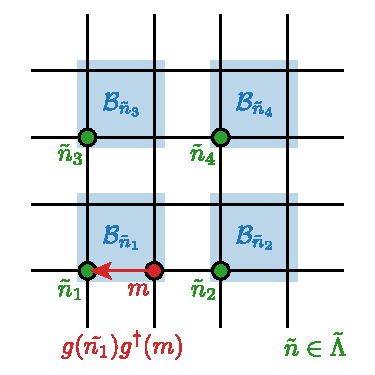
\includegraphics[width = 0.5\textwidth]{mg_averaging.pdf}
	\caption{Cartoon depiction for coarsening a gauge theory. The fine lattice is denoted by the black lines, and the coarse lattice points $\tilde{n}\in\tilde{\Lambda}$ are shown in green. Four blocks $\mathcal{B}_{\tilde{n}}$ are shown in this cartoon, each of which is shaded in blue. Averaging over each block is performed by parallel transporting each point $m$ in the block to its reference point $\tilde{n}$ with $g(\tilde{n}) g^\dagger(m) \psi(m)$, which is shown in red.}
	\label{fig:mg_coarsen_gt}
\end{figure}

%$\psi'(n)$ = fine grid prolongation from coarse field , where $m\in \mathcal B_{\tilde{n}}$
Prolongation from the coarse field $\tilde{\psi}(\tilde{n})$ to the fine field $\psi(n)$ can be defined in a similar way: one can use standard MG prolongation stencils and techniques, as long as the prolongated field transforms covariantly under gauge rotations on the fine lattice $\Lambda$. Suppose that $m\in\Lambda$ is contained in block $\mathcal B_{\tilde{n}}$. As a simple example, a piecewise-constant prolongation over each coarse-grid block has a fine field $\psi(m)$ taking the form
\begin{equation}
	\psi(m) = g(m) g^\dagger(\tilde{n}) \tilde{\psi}(\tilde{n}).
\end{equation}
In this case, one evaluates $\psi(m)$ by with the value of the coarse field at $\tilde{n}$, and then parallel transports the value appropriately to transform under gauge transformations at $m$ as it must. 

% Notation may be a bit imprecise here
Any standard prolongation operator can be defined respecting gauge invariance as long as the fields are correctly parallel transported with $g(n) g^\dagger(m)$ before being added together. For a general stencil $s(n, m)$ that defines the prolongation operator\footnote{For example, on a 2D grid, the stencil \begin{equation} s(n, m) \rightarrow \frac{1}{4} \left] \begin{matrix} 1 & 2 & 1 \\ 2 & 4 & 2 \\ 1 & 2 & 1 \end{matrix} \right[ \end{equation} that implements a 2D linear interpolation. }, the stencil can correctly take into account gauge invariance by being augmented with the correct gauge transformation,
\begin{equation}
	\psi(m) = \sum_{n\in\Lambda} s(m, n) g(m) g^\dagger(n) \tilde{\psi}(n).
\end{equation}
Here the coarse field $\tilde{\psi}(n)$ is defined on the fine lattice $n\in\Lambda$ with the canonical embedding,
\begin{equation}
	\tilde{\psi}(n) = \begin{cases} 
		\tilde{\psi}(n) & n\in\tilde{\Lambda} \\
		0 		    & n\notin \tilde{\Lambda} 
	\end{cases}.
\end{equation}
In the case where the gauge fixing matrix $g(n)$ is unity, or when we do not have to worry about a gauge field, this should reduce to the usual interpolation operator from the stencil $s(n, m)$. 


\chapter{General Cayley form}

Now consider a generalisation of the action that includes
both Tanh and Zolotarev approximations to  Moebius fermions
\cite{Brower:2004xi,Brower:2005qw}
which have Shamir and Neuberger kernels as limiting cases as
shown by Borici\cite{Borici:1999zw,Borici:1999da}.

\begin{equation}
S^5 = \bar{\psi} D^5_{GDW} \psi
\end{equation}
We define
\begin{eqnarray}
D^s_+ &=& \alpha_s (b_s  D_W + 1)\\
D^s_- &=& \alpha_s (1-c_s  D_W )\\
\tilde{D}^s &=& (D^s_-)^{-1} D^s_+
\end{eqnarray}
and take
\begin{eqnarray}
D^5_{GDW}
 &= &  (D_-)^{-1} D^5_{Brower}\\
 &= & 
 \left( 
         (D_-^{s})^{-1} D^{s}_+ \delta_{s,s^\prime}
 -  P_- \delta_{s,s^\prime-1}
 -  P_+ \delta_{s,s^\prime+1} 
\right) \\
&=&
\left(
\begin{array}{cccccc}
  (D^1_- )^{-1}D^1_+ & - P_- & 0& \ldots & 0 &  m P_+ \\
-  P_+  & \ddots &  \ddots & 0      & \ldots &0 \\
0     & \ddots &  \ddots & \ddots & 0      &\vdots \\
\vdots& 0      &  \ddots & \ddots & \ddots & 0\\
0     & \ldots &    0    &  \ddots& \ddots & - P_- \\
m P_- & 0      & \ldots  &  0     &   - P_+   
& (D^{L_s}_- )^{-1}D^{L_s}_+
\end{array}
\right)\\
&=&
\left(
\begin{array}{cccccc}
  \tilde{D}^{1} & - P_- & 0& \ldots & 0 &  m P_+ \\
-  P_+  & \ddots &  \ddots & 0      & \ldots &0 \\
0     & \ddots &  \ddots & \ddots & 0      &\vdots \\
\vdots& 0      &  \ddots & \ddots & \ddots & 0\\
0     & \ldots &    0    &  \ddots& \ddots & - P_- \\
m P_- & 0      & \ldots  &  0     &   - P_+   
& \tilde{D}^{L_s}
\end{array}
\right)
\end{eqnarray}

Standard Domain Wall Fermions correspond to $\alpha_s=1 ; b=1 ; c=0$ 

For a $\tanh$ approximation $b_s, c_s$ are constant and the matrix remains
translationally invariant in the fifth dimension (anti-periodic).

\begin{thebibliography}{99}

%\cite{Kaplan:1992bt}
\bibitem{Kaplan:1992bt}
  D.~B.~Kaplan,
  ``A Method for simulating chiral fermions on the lattice,''
  Phys.\ Lett.\ B {\bf 288} (1992) 342
  [hep-lat/9206013].
  %%CITATION = HEP-LAT/9206013;%%

\bibitem{Shamir:1993zy}
  Y.~Shamir,
  ``Chiral fermions from lattice boundaries,''
  Nucl.\ Phys.\ B {\bf 406} (1993) 90
  [hep-lat/9303005].
  %%CITATION = HEP-LAT/9303005;%%


\bibitem{Furman:1994ky}
  V.~Furman and Y.~Shamir,
  ``Axial symmetries in lattice QCD with Kaplan fermions,''
  Nucl.\ Phys.\ B {\bf 439} (1995) 54
  [hep-lat/9405004].
  %%CITATION = HEP-LAT/9405004;%%
%\cite{Blum:1996jf}
\bibitem{Blum:1996jf}
  T.~Blum and A.~Soni,
  ``QCD with domain wall quarks,''
  Phys.\ Rev.\ D {\bf 56} (1997) 174
  [hep-lat/9611030].
  %%CITATION = HEP-LAT/9611030;%%

%\cite{Narayanan:1993sk}
\bibitem{Narayanan:1993sk}
  R.~Narayanan and H.~Neuberger,
  ``Chiral determinant as an overlap of two vacua,''
  Nucl.\ Phys.\ B {\bf 412} (1994) 574
  [hep-lat/9307006].
  %%CITATION = HEP-LAT/9307006;%%

%\cite{Narayanan:1993ss}
\bibitem{Narayanan:1993ss}
  R.~Narayanan and H.~Neuberger,
  ``Chiral fermions on the lattice,''
  Phys.\ Rev.\ Lett.\  {\bf 71} (1993) 3251
  [hep-lat/9308011].
  %%CITATION = HEP-LAT/9308011;%%

%\cite{Narayanan:1994gw}
\bibitem{Narayanan:1994gw}
  R.~Narayanan and H.~Neuberger,
  ``A Construction of lattice chiral gauge theories,''
  Nucl.\ Phys.\ B {\bf 443} (1995) 305
  [hep-th/9411108].
  %%CITATION = HEP-TH/9411108;%%

%\cite{Neuberger:1997fp}
\bibitem{Neuberger:1997fp}
  H.~Neuberger,
  ``Exactly massless quarks on the lattice,''
  Phys.\ Lett.\ B {\bf 417} (1998) 141
  [hep-lat/9707022].
  %%CITATION = HEP-LAT/9707022;%%

% Domain wall equivalence


%
\bibitem{Neuberger:1997bg}
  H.~Neuberger,
  ``Vector - like gauge theories with almost massless fermions on the lattice,''
  Phys.\ Rev.\  D {\bf 57} (1998) 5417
  [arXiv:hep-lat/9710089].
  %%CITATION = PHRVA,D57,5417;%%
%\cite{Kikukawa:1999sy}
\bibitem{Kikukawa:1999sy}
  Y.~Kikukawa and T.~Noguchi,
  ``Low-energy effective action of domain wall fermion and the Ginsparg-Wilson relation,''
  hep-lat/9902022.
  %%CITATION = HEP-LAT/9902022;%%
%\cite{Edwards:2000qv}
\bibitem{Edwards:2000qv}
  R.~G.~Edwards and U.~M.~Heller,
  ``Domain wall fermions with exact chiral symmetry,''
  Phys.\ Rev.\ D {\bf 63} (2001) 094505
  [hep-lat/0005002].
  %%CITATION = HEP-LAT/0005002;%%

% Ginsparg Wilson

%\cite{Neuberger:1998wv}
\bibitem{Neuberger:1998wv}
  H.~Neuberger,
  ``More about exactly massless quarks on the lattice,''
  Phys.\ Lett.\ B {\bf 427} (1998) 353
  [hep-lat/9801031].
  %%CITATION = HEP-LAT/9801031;%%
%\cite{Luscher:1998pqa}
\bibitem{Luscher:1998pqa}
  M.~Luscher,
  ``Exact chiral symmetry on the lattice and the Ginsparg-Wilson relation,''
  Phys.\ Lett.\ B {\bf 428} (1998) 342
  [hep-lat/9802011].
  %%CITATION = HEP-LAT/9802011;%%



% Axial current
%\cite{Kikukawa:1998py}
\bibitem{Kikukawa:1998py}
  Y.~Kikukawa and A.~Yamada,
  ``Axial vector current of exact chiral symmetry on the lattice,''
  Nucl.\ Phys.\ B {\bf 547} (1999) 413
  [hep-lat/9808026].
  %%CITATION = HEP-LAT/9808026;%%
%\cite{Kikukawa:1998pd}
\bibitem{Kikukawa:1998pd}
  Y.~Kikukawa and A.~Yamada,
  ``Weak coupling expansion of massless QCD with a Ginsparg-Wilson fermion and axial U(1) anomaly,''
  Phys.\ Lett.\  B {\bf 448} (1999) 265
  [arXiv:hep-lat/9806013].
  %%CITATION = PHLTA,B448,265;%%

% Many kernels

%\cite{Borici:1999zw}
\bibitem{Borici:1999zw}
  A.~Borici,
  ``Truncated overlap fermions,''
  Nucl.\ Phys.\ Proc.\ Suppl.\  {\bf 83} (2000) 771
  [hep-lat/9909057].
  %%CITATION = HEP-LAT/9909057;%%
%\cite{Borici:1999da}
\bibitem{Borici:1999da}
  A.~Borici,
  ``Truncated overlap fermions: The Link between overlap and domain wall fermions,''
  hep-lat/9912040.
  %%CITATION = HEP-LAT/9912040;%%
%\cite{Borici:2004pn}
\bibitem{Borici:2004pn}
  A.~Borici,
  ``Computational methods for the fermion determinant and the link between overlap and domain wall fermions,''
  hep-lat/0402035.
  %%CITATION = HEP-LAT/0402035;%%


% Continued fraction

%\cite{Borici:2001ua}
\bibitem{Borici:2001ua}
  A.~Borici, A.~D.~Kennedy, B.~J.~Pendleton and U.~Wenger,
  ``The Overlap operator as a continued fraction,''
  Nucl.\ Phys.\ Proc.\ Suppl.\  {\bf 106} (2002) 757
  [hep-lat/0110070].
  %%CITATION = HEP-LAT/0110070;%%

%\cite{Edwards:2005an}
\bibitem{Edwards:2005an}
  R.~G.~Edwards, B.~Joo, A.~D.~Kennedy, K.~Orginos and U.~Wenger,
  ``Comparison of chiral fermion methods,''
  PoS LAT {\bf 2005} (2006) 146
  [hep-lat/0510086].
  %%CITATION = HEP-LAT/0510086;%%

%CHROMA
%\cite{Edwards:2004sx}
\bibitem{Edwards:2004sx}
  R.~G.~Edwards {\it et al.}  [SciDAC and LHPC and UKQCD Collaborations],
  ``The Chroma software system for lattice QCD,''
  Nucl.\ Phys.\ Proc.\ Suppl.\  {\bf 140} (2005) 832
  [hep-lat/0409003].
  %%CITATION = HEP-LAT/0409003;%%


\bibitem{Kennedy:2006ax}
  A.~D.~Kennedy,
  ``Algorithms for dynamical fermions,''
  hep-lat/0607038.
  %%CITATION = HEP-LAT/0607038;%%.
%\cite{Antonio:2008zz}
\bibitem{Antonio:2008zz}
  D.~J.~Antonio {\it et al.}  [RBC and UKQCD Collaborations],
  ``Localization and chiral symmetry in three flavor domain wall QCD,''
  Phys.\ Rev.\ D {\bf 77} (2008) 014509
  [arXiv:0705.2340 [hep-lat]].
  %%CITATION = ARXIV:0705.2340;%%

%\cite{Brower:2004xi}
\bibitem{Brower:2004xi}
  R.~C.~Brower, H.~Neff and K.~Orginos,
  ``Mobius fermions: Improved domain wall chiral fermions,''
  Nucl.\ Phys.\ Proc.\ Suppl.\  {\bf 140} (2005) 686
  [hep-lat/0409118].
  %%CITATION = HEP-LAT/0409118;%%

%\cite{Brower:2005qw}
\bibitem{Brower:2005qw}
  R.~C.~Brower, H.~Neff and K.~Orginos,
  ``Mobius fermions,''
  Nucl.\ Phys.\ Proc.\ Suppl.\  {\bf 153} (2006) 191
  [hep-lat/0511031].
  %%CITATION = HEP-LAT/0511031;%%
\bibitem{Narayanan:2000qx}
  R.~Narayanan and H.~Neuberger,
  ``An Alternative to domain wall fermions,''
  Phys.\ Rev.\ D {\bf 62} (2000) 074504
  [hep-lat/0005004].
  %%CITATION = HEP-LAT/0005004;%%

\bibitem{BAGEL}
Peter A. Boyle
``The BAGEL assembler generation library''
Computer Physics Communications, Volume 180, Issue 12, December 2009, Pages 2739-2748
\end{thebibliography}



\end{document}

\subsection{Pseudofermion action for CF and PF}

Here we deal exclusively with 4d pseudofermions, and 
the pseudofermion action is simple and involves no Pauli Villars fields:

\begin{eqnarray}
S_{PF} &=&  (0,\ldots, 0,\phi^\dagger) [(D_\chi^5)^\dagger D_\chi^5]^{-1}
(0,\ldots, 0,\phi)^T\nonumber\\
&=&
 (0,\ldots, 0,\phi^\dagger) U^{-1} 
{\rm diag}( D_1^{-1},\ldots, D_{N-1}^{-1}, R(H)^{-1})
L^{-1}U^{-\dagger} 
{\rm diag}( D_1^{-\dagger},\ldots, D_{N-1}^{-\dagger}, R(H)^{-\dagger})
L^{-\dagger}(0,\ldots, 0,\phi)^T\nonumber\\
&=&
(0,\ldots, 0,\phi^\dagger) U^\prime
(X_1,\ldots,X_{N-1} ,[R(H)^\dagger R(H)]^{-1}\phi)^T\nonumber\\
&=& \phi^\dagger [R(H)^\dagger R(H)]^{-1}\phi\nonumber\\
&\equiv&
\phi^\dagger 
(D_{ov}^\dagger D_{ov})^{-1}
\phi\nonumber
\end{eqnarray}

Conclusions:

The CF and PF forms look cleaner in HMC with
no Pauli Villars needed, and naturally fit with 4d pseudofermions.
The PF and CF allow relaxed approximation during 
molecular dynamics compared to accept reject.

However, one must perform two sequential solves to 
